%%%%%%%%%%%%%%%%%%%%%%%%%%%%%%%%%%%%%%%%%%%%%%
%                insertmeeting
% 1) Title (something creative & funny?)
% 2) Date (MM/DD/YYYY)
% 3) Location (ex. Hagerty High School)
% 4) People/Committees Present 
% 5) Picture 
% 6) Start Time & Stop Time (ex. 12:30AM to 4:30PM)
%%%%%%%%%%%%%%%%%%%%%%%%%%%%%%%%%%%%%%%%%%%%%%
\insertmeeting 
	{Silly SDKs} 
	{10/01/21} 
	{Hagerty High School}
	{James, Jensen, Ritam, Samantha}
	{Images/RobotPics/robot.jpg}
	{2:30 - 4:30}
	
\hhscommittee{Software}
\noindent\hfil\rule{\textwidth}{.4pt}\hfil
\subsubsection*{Goals}
\begin{itemize}
    \item Bring Freight Frenzy SDK into our current repository

\end{itemize} 

\noindent\hfil\rule{\textwidth}{.4pt}\hfil

\subsubsection*{Accomplishments}
Woohoo! The FTC SDK is out! This meant that we had to do our yearly merge which consisted of 195 files this year. Because we use an external library called TRC, it becomes extremely difficult to make sure everything turns out okay. Funny enough, there was also an update for the TRC library which consisted of new classes and modification to old ones. 

We started to look into the depths of the new library and added the Hardware Mapping and set up the configuration as well. We are looking forward to this exciting new year!
 


\begin{figure}[htp]
\centering
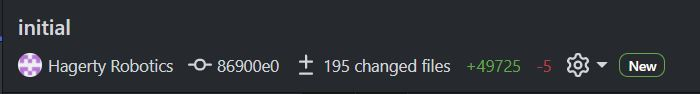
\includegraphics[width=0.95\textwidth, angle=0]{Meetings/October/10-01-21/10-19-21 - Ritam R.JPG}
\caption{First commit}
\label{fig:100121_1}
\end{figure}



\whatsnext{
\begin{itemize}
    \item Add classes for functional mechanisms
\end{itemize} 
}

